% This is part of Un soupçon de mathématique sans être agressif pour autant
% Copyright (c) 2012
%   Laurent Claessens
% See the file fdl-1.3.txt for copying conditions.

\chapter{Proportions, pourcentages}

%+++++++++++++++++++++++++++++++++++++++++++++++++++++++++++++++++++++++++++++++++++++++++++++++++++++++++++++++++++++++++++
\section{Théorie}
%+++++++++++++++++++++++++++++++++++++++++++++++++++++++++++++++++++++++++++++++++++++++++++++++++++++++++++++++++++++++++++

Nous disons qu'un gaz est en concentration de une \defe{partie par million}{partie par million} si un million de grammes d'air contient un gramme du gaz. Voici quelque chiffre concernant l'évolution de la concentration de \( CO_2\) dans l'atmosphère; les chiffres sont en \( \unit{}{ppm}\) :
\begin{center}
\begin{tabular}{|c|c|c|}
    \hline
    1750    &   2005    &   1012\\
    \hline
    280&380&395\\
    \hline
\end{tabular}
\end{center}
Pour information, cette concentration n'a pas dépassé les \unit{300}{ppm} depuis au moins \( 600.000\) ans.

\begin{enumerate}
    \item
        De combien de pourcent la concentration de \( CO_2\) a augmenté entre 1750 et 2005 ?
    \item
        Sur un kilo d'air, combien de grammes de \( CO_2\) ?
    \item 
        Quelle est la vitesse (en ppm par an) d'augmentation de la concentration entre 1750 et 2005 ? Même question entre 2005 et 2012.
\end{enumerate}

\begin{definition}
    Une \defe{population}{population} est un ensemble fini. Si \( E\) est une population, une \defe{sous-population}{sous-population} est un sous-ensemble \( A\subset E\). L'\defe{effectif}{effectif} d'une population est le nombre de ses éléments.

    La \defe{proportion}{proportion} de \( A\) dans \( E\) est le rapport
    \begin{equation}
        p_A=\frac{ n_A }{ n_E }
    \end{equation}
    où \( n_A\) et \( n_E\) sont les effectifs de \( A\) et \( E\).
\end{definition}
Note : une proportion est un nombre compris entre zéro et un.

\begin{example}
    Demander combien il y a de gauchers dans la classe. Quelle en est la proportion ?
\end{example}

\begin{example}
    Diviser la classe en \( 4\) groupes suivant que l'élève habite ou non à Dole et qu'il utilise ou non un cahier. Remplir le tableau suivant :

    \begin{center}
    \begin{tabular}{|l||c|c||c|}
        \hline\hline
        & habite à Dole&n'habite pas à Dole&total\\
        \hline
        utilise un cahier&&&\\
        \hline
        n'utilise pas de cahier&&&\\
        \hline\hline
        total&&&\\
        \hline
    \end{tabular}
    \end{center}

    Soit \( E\) la population totale : toute la classe; soit $A$ la population de ceux qui vivent à Dole; et \( B\) celle de ceux qui utilisent un cahier.
    \begin{enumerate}
        \item
            Trouver les effectifs des populations \( A\cup B\) et \( A\cap B\).
        \item
            Quelle est la proportion de \( A\) dans \( E\) ? Et celle du complémentaire \( \bar A\) ?
        \item
            Exprimer les proportions \( p_{A\cap B}\) et \( p_{A\cup B}\).
    \end{enumerate}
\end{example}

Nous avons l'égalité
\begin{equation}
    n_{A\cup B}=n_A+n_B-n_{A\cap B}
\end{equation}
parce que dans le compte \( n_A+n_B\), nous comptons deux fois les individus qui sont dans \( A\) et dans \( B\). En passant aux proportions (c'est à dire en divisant tout par \( n_E\)), nous avons la formule
\begin{equation}
    p_{A\cup B}=p_A+p_B-p_{A\cap B}.
\end{equation}

\begin{remark}
    Si les populations \( A\) et \( B\) sont disjointes, alors \( n_{A\cap B}=0\) et nous trouvons la formule
    \begin{equation}
        p_{A\cup B}=p_A+p_B.
    \end{equation}
\end{remark}


%+++++++++++++++++++++++++++++++++++++++++++++++++++++++++++++++++++++++++++++++++++++++++++++++++++++++++++++++++++++++++++
\section{Exercices}
%+++++++++++++++++++++++++++++++++++++++++++++++++++++++++++++++++++++++++++++++++++++++++++++++++++++++++++++++++++++++++++

\Exo{Seconde-0022}
\Exo{Seconde-0030}
\Exo{Premiere-0001}
\Exo{Premiere-0002}
\Exo{Premiere-0003}
\Exo{Premiere-0004}
\Exo{Premiere-0005}
\Exo{Premiere-0006}

\Exo{Premiere-0007}
\Exo{Premiere-0008}
\Exo{Premiere-0009}
\Exo{Premiere-0010}
\Exo{Premiere-0011}
\Exo{Premiere-0012}
\Exo{Seconde-0026}
\Exo{Seconde-0024}
\Exo{Premiere-0014}                                                                                                                                     
\Exo{Premiere-0015}                                               
\Exo{Premiere-0016}                                                                       
\Exo{Premiere-0017}                                                                                                                      
\Exo{Seconde-0034}

\Exo{Premiere-0023}                                                                                                                                    


\chapter{Second degré}

%+++++++++++++++++++++++++++++++++++++++++++++++++++++++++++++++++++++++++++++++++++++++++++++++++++++++++++++++++++++++++++
\section{Définitions}
%+++++++++++++++++++++++++++++++++++++++++++++++++++++++++++++++++++++++++++++++++++++++++++++++++++++++++++++++++++++++++++

\begin{definition}
    Une fonction \defe{polynôme de degré $2$}{polynôme (de degré $2$)} est une fonction s'exprimant sous la forme 
    \begin{equation}
    f(x)=ax^2+bx+c
    \end{equation}
    où \( a\), \( b\) et \( c\) sont des nombres réels avec \( a\neq 0\). 
    
    La courbe représentative d'un polynôme de degré deux dans un plan orthonormé est une \defe{parabole}{parabole}.
\end{definition}

%---------------------------------------------------------------------------------------------------------------------------
\subsection{Symétries, tableau de variations}
%---------------------------------------------------------------------------------------------------------------------------

La parabole de la fonction \( f(x)=ax^2+bx+c\) (\( a\neq 0\)) est symétrique par rapport à la droite d'équation \( x=-\frac{ b }{ 2a }\), c'est à dire par rapport à la droite verticale en \( x=-b/2a\). Le \defe{sommet}{sommet (d'une parabole)} est le point d'abscisse 
\begin{equation}
x=-b/2a
\end{equation}
situé sur la parabole.

Deux paraboles avec leurs axes de symétries sont dessinées à la figure \ref{LabelFigParaboles}.
\newcommand{\CaptionFigParaboles}{Deux paraboles}
\input{Fig_Paraboles.pstricks}

Comment savoir si les branches de la paraboles \( ax^2+bx+c\) sont orientées vers le haut ou vers le bas ? La règle est simple : 
\begin{enumerate}
    \item
        si \( a>0\), alors elles sont tournées vers le haut;
    \item
        si \( a<0\), alors elles sont tournées vers le bas.
\end{enumerate}
Cette règle est facile à retenir en pensant par exemple à la parabole \( x^2+bx+c\) où \( b\) et \( c\) sont raisonnables. Si nous prenons \( x=1000\), alors \( x^2\) vaut un million alors que les deux autres termes ne valent que de l'ordre du mille. Il est alors clair que la branche part vers l'infini.

\vbox{  % Le problème est que ceci apparaît proche du bord inférieur de la page, du coup il saut de colonne avant mon \columnbreak et l'effet est merdé.
\begin{multicols}{2}
    
    Le tableau de variations pour une parabole \( f(x)=ax^2+bx+c\) avec \( a>0\) se présente ainsi :
\begin{equation*}
\begin{array}[h]{|c||ccccc|}
    \hline
    x&-\infty&&x_0=-b/2a&&\infty\\
    \hline
    &\infty&&&&\infty\\
    f(x)&&\searrow&&\nearrow&\\
    &&&f(x_0)&&\\
    \hline
\end{array}
\end{equation*}

  \columnbreak

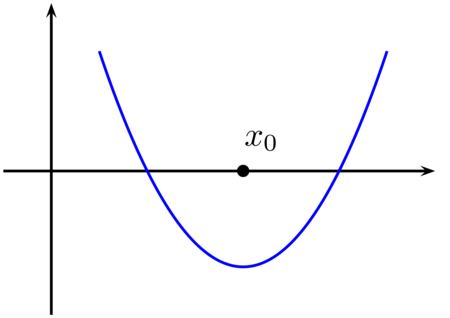
\includegraphics{Picture_FIGLabelFigParaboleHautMLbPQFPICTParaboleHautMLbPQF-for_eps.pdf}

\end{multicols}

}

\vbox{ 
\begin{multicols}{2}
    
    Le tableau de variations pour une parabole \( f(x)=ax^2+bx+c\) avec \( a<0\) se présente ainsi :
\begin{equation*}
\begin{array}[h]{|c||ccccc|}
    \hline
    x&-\infty&&x_0=-b/2a&&\infty\\
    \hline
    &&&f(x_0)&&\\
    f(x)&&\nearrow&&\searrow&\\
    &-\infty&&&&-\infty\\
    \hline
\end{array}
\end{equation*}


  \columnbreak

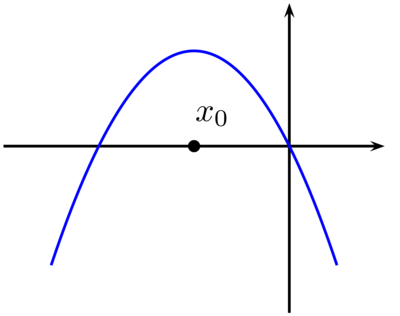
\includegraphics{Picture_FIGLabelFigParaboleBasfKtFCNPICTParaboleBasfKtFCN-for_eps.pdf}
\end{multicols}

}

%+++++++++++++++++++++++++++++++++++++++++++++++++++++++++++++++++++++++++++++++++++++++++++++++++++++++++++++++++++++++++++
\section{Tracer une parabole dont l'équation est connue}
%+++++++++++++++++++++++++++++++++++++++++++++++++++++++++++++++++++++++++++++++++++++++++++++++++++++++++++++++++++++++++++

Maintenant que les symétrie de la paraboles sont sont connues, il devient relativement facile d'en dessiner. Il est important d'être capable de tracer à main levée une courbe approximative passant par quelque points connus. SANS CALCULATRICE\footnote{Si vous me permettez une analogie, utiliser une calculatrice pour faire des études de fonctions, c'est comme utiliser un anti douleur pour améliorer ses performances sportives.}.

La méthode pour tracer la courbe représentative de \( f(x)=ax^2+bx+c\) se décompose en les pas suivants.
\begin{enumerate}
    \item
        D'abord il faut trouver le sommet de la parabole en utilisant la formule 
        \begin{equation}
            x_0=-\frac{ b }{ 2a }.
        \end{equation}
        Le somme est alors le point \( S=\big( x_0,f(x_0) \big)\).
    \item
        Tracer la droite verticale passant par le sommet; ce sera l'axe de symétrie.
    \item
        Dresser le tableau de variations de \( f\) en regardant le signe de \( a\). Si \( a\) est positif, le sommet sera le creux de la courbe; si \( a\) est négatif, alors le sommet sera un pic du graphique.
    \item
        Calculer quelque valeurs autour du sommet, par exemple \( x=0\), \( x=\pm1\).
    \item
        Tracer une belle courbe passant par les points calculés, ayant le bon axe de symétrie et le bon sommet.
\end{enumerate}

\begin{example}
    Traçons la courbe représentative de \( f(x)=x^2\). Ses paramètres sont \( a=1\), \( b=0\), \( c=0\); son axe de symétrie est donc \( x=0\), c'est à dire l'axe des ordonnées. Son sommet est le point \( S=(0,0)\) et le graphe passe par les points \( (-2,4)\), \( (-1,1)\), \( (0,0)\), \( (2,4)\). En repérant ces points sur la feuille, le tracé est aisé.

    Attention : c'est une courbe qui monte assez fort. Elle est tracée sur la figure \ref{LabelFigbDdpfh}.
\newcommand{\CaptionFigbDdpfh}{La courbe \( x\mapsto x^2\).}
\input{Fig_bDdpfh.pstricks}

\end{example}

\begin{example}
    Soit à tracer la courbe de \( f(x)=x^2-4x+3\).
    \begin{enumerate}
        \item
            Nous identifions \( a=1\), \( b=-4\), \( c=3\). 
        \item
            L'abscisse du sommet est \( x_0=-b/2a=\frac{ 4 }{2}=2\). Étant donné que \( f(2)=4-8+3=-1\), le sommet est en \( S=(2,-1)\).
        \item
            Calculons quelque points :
            \begin{itemize}
                \item \( f(1)=0\),
                \item
                    \( f(3)=0\),
                \item
                    \( f(0)=3\),
                \item
                    \( f(4)=3\).
            \end{itemize}
            Il est important de résister à la tentation de faire cette étape à la calculatrice tant que vous n'êtes pas complètement à l'aise.
        \item
            Placer les points \( (2,-1)\), \( (1,0)\), \( (3,0)\), \( (0,3)\) et \( (4,3)\) dans un plan.
        \item
            Tracer.
    \end{enumerate}
    Le résultat est tracé sur la figure \ref{LabelFigParabolevQzhjq}.
\newcommand{\CaptionFigParabolevQzhjq}{La courbe de la parabole \( x^2-4x+3\).}
\input{Fig_ParabolevQzhjq.pstricks}
\end{example}

\begin{example}
    Traçons la courbe de \( -x^2+4\). Une bonne chose à faire est de remarquer que cela est un produit remarquable :
    \begin{equation}
        f(x)=-(x+2)(x-2).
    \end{equation}
    Ceci va un peu nous simplifier la tâche parce que nous savons immédiatement les racines\footnote{Notons que nous n'avons pas encore montré comment trouver en général les racines d'un polynôme du second degré.} : \( \pm2\).
    %TODO : ajouter un lien vers là où ce sera fait

    Le sommet est en \( x_0=0\) et donc le sommet est \( S=(0,4)\). Nous pouvons encore calculer les points \( f(1)=3\) et \( f(3)=-5\). Avec cela nous pouvons tracer.

Le résultat est à la figure \ref{LabelFigParaboleiLbviP}.
\newcommand{\CaptionFigParaboleiLbviP}{La courbe de \( -x^2+4=-(x+2)(x-2)\).}
\input{Fig_ParaboleiLbviP.pstricks}

\end{example}

% TODO : À mettre quelque part : retenir que «parabole», «trinôme» et «polynôme du second degré», ce sont trois expressions essentiellement équivalentes.

%+++++++++++++++++++++++++++++++++++++++++++++++++++++++++++++++++++++++++++++++++++++++++++++++++++++++++++++++++++++++++++
\section{Donner l'équation d'une parabole dont deux racines sont connues}
%+++++++++++++++++++++++++++++++++++++++++++++++++++++++++++++++++++++++++++++++++++++++++++++++++++++++++++++++++++++++++++

\begin{example}
    Trouver une parabole qui s'annule en \( x=3\) et \( x=8\). Cela est très simple : il suffit d'écrire
    \begin{equation}
        f(x)=(x-3)(x-8).
    \end{equation}
    Le fait que cela s'annule en \( x=3\) et \( x=5\) est immédiat. En développant nous pouvons également l'écrire
    \begin{equation}
        f(x)=(x-3)(x-8)=x^2-8x-3x+24=x^2-11x+24.
    \end{equation}
    Le sommet de cette parabole est \( 11/2=5.5\). Remarquons encore que \( 5.5\) est juste au milieu de \( 3\) et \( 8\).
\end{example}

\begin{Aretenir}
    Les polynômes du second degré s'annulant en \( x=x_1\) et en \( x=x_2\) s'écrivent 
    \begin{equation}
        f(x)=m(x-x_1)(x-x_2)
    \end{equation}
    où \( m\) est n'importe quel réel.
\end{Aretenir}

Attention aux signes. Un polynôme qui s'annule en \( x=-1\) et \( x=-5\) s'écrit \( m(x+1)(x+5)\).

\begin{example}
    Un polynôme du second degré s'annulant en \( x=1\), en \( x=-2\) et dont le sommet est à la hauteur \( 5\). D'abord nous écrivons la forme générale du polynôme s'annulant en \( x=1\) et \( x=-2\) :
    \begin{equation}
        f(x)=m(x-1)(x+2).
    \end{equation}
    Nous développons : \( f(x)=m\big( x^2+x-2 \big)\). Le sommet de cette parabole est en \( x_S=-1/2\); notez que cela ne dépend pas de \( m\). Le sommet de la parabole est donc à la hauteur
    \begin{subequations}
        \begin{align}
            f(x_S)&=f\left( -\frac{ 1 }{2}j \right)\\
            &=m\Big( \left( -\frac{ 1 }{2} \right)^2+\frac{ 1 }{2}-2 \Big)\\
            &=m\Big( \frac{1}{ 4 }+\frac{1}{ 2 }-2 \Big)\\
            &=-\frac{ 5m }{ 4 }.
        \end{align}
    \end{subequations}
    Nous devons fixer \( m\) pour que cette hauteur soit \( 5\), c'est à dire résoudre
    \begin{equation}
        -\frac{ 5m }{ 4 }=5,
    \end{equation}
    la solution est \( m=-4\). En définitive la fonction recherchée est
    \begin{equation}
        f(x)=-4x^2+4x-8.
    \end{equation}
\end{example}

%+++++++++++++++++++++++++++++++++++++++++++++++++++++++++++++++++++++++++++++++++++++++++++++++++++++++++++++++++++++++++++
\section{Exercices sur le second degré}
%+++++++++++++++++++++++++++++++++++++++++++++++++++++++++++++++++++++++++++++++++++++++++++++++++++++++++++++++++++++++++++

\Exo{Premiere-0030}
\Exo{Premiere-0031}
\Exo{Premiere-0032}

\Exo{Premiere-0041}
\Exo{Premiere-0024}                                                                                                                                  
\Exo{Premiere-0040}
\Exo{Premiere-0026}                                                                                               

%---------------------------------------------------------------------------------------------------------------------------
\subsection{Plus compliqués}
%---------------------------------------------------------------------------------------------------------------------------

\Exo{Premiere-0025}                                                                                                                                   
\Exo{Premiere-0028}
\Exo{Premiere-0029}
